\documentclass[1p]{elsarticle_modified}
%\bibliographystyle{elsarticle-num}

%\usepackage[colorlinks]{hyperref}
%\usepackage{abbrmath_seonhwa} %\Abb, \Ascr, \Acal ,\Abf, \Afrak
\usepackage{amsfonts}
\usepackage{amssymb}
\usepackage{amsmath}
\usepackage{amsthm}
\usepackage{scalefnt}
\usepackage{amsbsy}
\usepackage{kotex}
\usepackage{caption}
\usepackage{subfig}
\usepackage{color}
\usepackage{graphicx}
\usepackage{xcolor} %% white, black, red, green, blue, cyan, magenta, yellow
\usepackage{float}
\usepackage{setspace}
\usepackage{hyperref}

\usepackage{tikz}
\usetikzlibrary{arrows}

\usepackage{multirow}
\usepackage{array} % fixed length table
\usepackage{hhline}

%%%%%%%%%%%%%%%%%%%%%
\makeatletter
\renewcommand*\env@matrix[1][\arraystretch]{%
	\edef\arraystretch{#1}%
	\hskip -\arraycolsep
	\let\@ifnextchar\new@ifnextchar
	\array{*\c@MaxMatrixCols c}}
\makeatother %https://tex.stackexchange.com/questions/14071/how-can-i-increase-the-line-spacing-in-a-matrix
%%%%%%%%%%%%%%%

\usepackage[normalem]{ulem}

\newcommand{\msout}[1]{\ifmmode\text{\sout{\ensuremath{#1}}}\else\sout{#1}\fi}
%SOURCE: \msout is \stkout macro in https://tex.stackexchange.com/questions/20609/strikeout-in-math-mode

\newcommand{\cancel}[1]{
	\ifmmode
	{\color{red}\msout{#1}}
	\else
	{\color{red}\sout{#1}}
	\fi
}

\newcommand{\add}[1]{
	{\color{blue}\uwave{#1}}
}

\newcommand{\replace}[2]{
	\ifmmode
	{\color{red}\msout{#1}}{\color{blue}\uwave{#2}}
	\else
	{\color{red}\sout{#1}}{\color{blue}\uwave{#2}}
	\fi
}

\newcommand{\Sol}{\mathcal{S}} %segment
\newcommand{\D}{D} %diagram
\newcommand{\A}{\mathcal{A}} %arc


%%%%%%%%%%%%%%%%%%%%%%%%%%%%%5 test

\def\sl{\operatorname{\textup{SL}}(2,\Cbb)}
\def\psl{\operatorname{\textup{PSL}}(2,\Cbb)}
\def\quan{\mkern 1mu \triangleright \mkern 1mu}

\theoremstyle{definition}
\newtheorem{thm}{Theorem}[section]
\newtheorem{prop}[thm]{Proposition}
\newtheorem{lem}[thm]{Lemma}
\newtheorem{ques}[thm]{Question}
\newtheorem{cor}[thm]{Corollary}
\newtheorem{defn}[thm]{Definition}
\newtheorem{exam}[thm]{Example}
\newtheorem{rmk}[thm]{Remark}
\newtheorem{alg}[thm]{Algorithm}

\newcommand{\I}{\sqrt{-1}}
\begin{document}

%\begin{frontmatter}
%
%\title{Boundary parabolic representations of knots up to 8 crossings}
%
%%% Group authors per affiliation:
%\author{Yunhi Cho} 
%\address{Department of Mathematics, University of Seoul, Seoul, Korea}
%\ead{yhcho@uos.ac.kr}
%
%
%\author{Seonhwa Kim} %\fnref{s_kim}}
%\address{Center for Geometry and Physics, Institute for Basic Science, Pohang, 37673, Korea}
%\ead{ryeona17@ibs.re.kr}
%
%\author{Hyuk Kim}
%\address{Department of Mathematical Sciences, Seoul National University, Seoul 08826, Korea}
%\ead{hyukkim@snu.ac.kr}
%
%\author{Seokbeom Yoon}
%\address{Department of Mathematical Sciences, Seoul National University, Seoul, 08826,  Korea}
%\ead{sbyoon15@snu.ac.kr}
%
%\begin{abstract}
%We find all boundary parabolic representation of knots up to 8 crossings.
%
%\end{abstract}
%\begin{keyword}
%    \MSC[2010] 57M25 
%\end{keyword}
%
%\end{frontmatter}

%\linenumbers
%\tableofcontents
%
\newcommand\colored[1]{\textcolor{white}{\rule[-0.35ex]{0.8em}{1.4ex}}\kern-0.8em\color{red} #1}%
%\newcommand\colored[1]{\textcolor{white}{ #1}\kern-2.17ex	\textcolor{white}{ #1}\kern-1.81ex	\textcolor{white}{ #1}\kern-2.15ex\color{red}#1	}

{\Large $\underline{12a_{1011}~(K12a_{1011})}$}

\setlength{\tabcolsep}{10pt}
\renewcommand{\arraystretch}{1.6}
\vspace{1cm}\begin{tabular}{m{100pt}>{\centering\arraybackslash}m{274pt}}
\multirow{5}{120pt}{
	\centering
	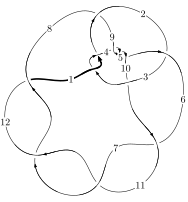
\includegraphics[width=112pt]{../../../GIT/diagram.site/Diagrams/png/1812_12a_1011.png}\\
\ \ \ A knot diagram\footnotemark}&
\allowdisplaybreaks
\textbf{Linearized knot diagam} \\
\cline{2-2}
 &
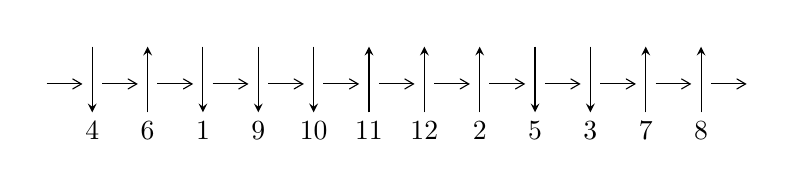
\begin{tikzpicture}[x=20pt, y=17pt]
	% nodes
	\node (C0) at (0, 0) {};
	\node (C1) at (1, 0) {};
	\node (C1U) at (1, +1) {};
	\node (C1D) at (1, -1) {4};

	\node (C2) at (2, 0) {};
	\node (C2U) at (2, +1) {};
	\node (C2D) at (2, -1) {6};

	\node (C3) at (3, 0) {};
	\node (C3U) at (3, +1) {};
	\node (C3D) at (3, -1) {1};

	\node (C4) at (4, 0) {};
	\node (C4U) at (4, +1) {};
	\node (C4D) at (4, -1) {9};

	\node (C5) at (5, 0) {};
	\node (C5U) at (5, +1) {};
	\node (C5D) at (5, -1) {10};

	\node (C6) at (6, 0) {};
	\node (C6U) at (6, +1) {};
	\node (C6D) at (6, -1) {11};

	\node (C7) at (7, 0) {};
	\node (C7U) at (7, +1) {};
	\node (C7D) at (7, -1) {12};

	\node (C8) at (8, 0) {};
	\node (C8U) at (8, +1) {};
	\node (C8D) at (8, -1) {2};

	\node (C9) at (9, 0) {};
	\node (C9U) at (9, +1) {};
	\node (C9D) at (9, -1) {5};

	\node (C10) at (10, 0) {};
	\node (C10U) at (10, +1) {};
	\node (C10D) at (10, -1) {3};

	\node (C11) at (11, 0) {};
	\node (C11U) at (11, +1) {};
	\node (C11D) at (11, -1) {7};

	\node (C12) at (12, 0) {};
	\node (C12U) at (12, +1) {};
	\node (C12D) at (12, -1) {8};
	\node (C13) at (13, 0) {};

	% arrows
	\draw[->,>={angle 60}]
	(C0) edge (C1) (C1) edge (C2) (C2) edge (C3) (C3) edge (C4) (C4) edge (C5) (C5) edge (C6) (C6) edge (C7) (C7) edge (C8) (C8) edge (C9) (C9) edge (C10) (C10) edge (C11) (C11) edge (C12) (C12) edge (C13) ;	\draw[->,>=stealth]
	(C1U) edge (C1D) (C2D) edge (C2U) (C3U) edge (C3D) (C4U) edge (C4D) (C5U) edge (C5D) (C6D) edge (C6U) (C7D) edge (C7U) (C8D) edge (C8U) (C9U) edge (C9D) (C10U) edge (C10D) (C11D) edge (C11U) (C12D) edge (C12U) ;
	\end{tikzpicture} \\
\hhline{~~} \\& 
\textbf{Solving Sequence} \\ \cline{2-2} 
 &
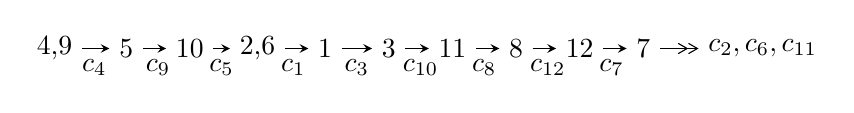
\begin{tikzpicture}[x=23pt, y=7pt]
	% node
	\node (A0) at (-1/8, 0) {4,9};
	\node (A1) at (1, 0) {5};
	\node (A2) at (2, 0) {10};
	\node (A3) at (49/16, 0) {2,6};
	\node (A4) at (33/8, 0) {1};
	\node (A5) at (41/8, 0) {3};
	\node (A6) at (49/8, 0) {11};
	\node (A7) at (57/8, 0) {8};
	\node (A8) at (65/8, 0) {12};
	\node (A9) at (73/8, 0) {7};
	\node (C1) at (1/2, -1) {$c_{4}$};
	\node (C2) at (3/2, -1) {$c_{9}$};
	\node (C3) at (5/2, -1) {$c_{5}$};
	\node (C4) at (29/8, -1) {$c_{1}$};
	\node (C5) at (37/8, -1) {$c_{3}$};
	\node (C6) at (45/8, -1) {$c_{10}$};
	\node (C7) at (53/8, -1) {$c_{8}$};
	\node (C8) at (61/8, -1) {$c_{12}$};
	\node (C9) at (69/8, -1) {$c_{7}$};
	\node (A10) at (11, 0) {$c_{2},c_{6},c_{11}$};

	% edge
	\draw[->,>=stealth]	
	(A0) edge (A1) (A1) edge (A2) (A2) edge (A3) (A3) edge (A4) (A4) edge (A5) (A5) edge (A6) (A6) edge (A7) (A7) edge (A8) (A8) edge (A9) ;
	\draw[->>,>={angle 60}]	
	(A9) edge (A10);
\end{tikzpicture} \\ 

\end{tabular} \\

\footnotetext{
The image of knot diagram is generated by the software ``\textbf{Draw programme}" developed by Andrew Bartholomew(\url{http://www.layer8.co.uk/maths/draw/index.htm\#Running-draw}), where we modified some parts for our purpose(\url{https://github.com/CATsTAILs/LinksPainter}).
}\phantom \\ \newline 
\centering \textbf{Ideals for irreducible components\footnotemark of $X_{\text{par}}$} 
 
\begin{align*}
I^u_{1}&=\langle 
-7.77473\times10^{61} u^{59}-1.16877\times10^{62} u^{58}+\cdots+1.10219\times10^{62} b+6.06781\times10^{61},\\
\phantom{I^u_{1}}&\phantom{= \langle  }-4.84379\times10^{62} u^{59}-8.34198\times10^{62} u^{58}+\cdots+1.10219\times10^{62} a-4.12695\times10^{62},\;u^{60}+3 u^{59}+\cdots-3 u^2+1\rangle \\
\\
\end{align*}
\raggedright * 1 irreducible components of $\dim_{\mathbb{C}}=0$, with total 60 representations.\\
\footnotetext{All coefficients of polynomials are rational numbers. But the coefficients are sometimes approximated in decimal forms when there is not enough margin.}
\newpage
\renewcommand{\arraystretch}{1}
\centering \section*{I. $I^u_{1}= \langle -7.77\times10^{61} u^{59}-1.17\times10^{62} u^{58}+\cdots+1.10\times10^{62} b+6.07\times10^{61},\;-4.84\times10^{62} u^{59}-8.34\times10^{62} u^{58}+\cdots+1.10\times10^{62} a-4.13\times10^{62},\;u^{60}+3 u^{59}+\cdots-3 u^2+1 \rangle$}
\flushleft \textbf{(i) Arc colorings}\\
\begin{tabular}{m{7pt} m{180pt} m{7pt} m{180pt} }
\flushright $a_{4}=$&$\begin{pmatrix}1\\0\end{pmatrix}$ \\
\flushright $a_{9}=$&$\begin{pmatrix}0\\u\end{pmatrix}$ \\
\flushright $a_{5}=$&$\begin{pmatrix}1\\u^2\end{pmatrix}$ \\
\flushright $a_{10}=$&$\begin{pmatrix}- u\\- u^3+u\end{pmatrix}$ \\
\flushright $a_{2}=$&$\begin{pmatrix}4.39469 u^{59}+7.56854 u^{58}+\cdots+8.66548 u+3.74431\\0.705389 u^{59}+1.06041 u^{58}+\cdots-0.422370 u-0.550522\end{pmatrix}$ \\
\flushright $a_{6}=$&$\begin{pmatrix}- u^2+1\\- u^4+2 u^2\end{pmatrix}$ \\
\flushright $a_{1}=$&$\begin{pmatrix}5.10008 u^{59}+8.62895 u^{58}+\cdots+8.24311 u+3.19379\\0.705389 u^{59}+1.06041 u^{58}+\cdots-0.422370 u-0.550522\end{pmatrix}$ \\
\flushright $a_{3}=$&$\begin{pmatrix}4.47039 u^{59}+7.66384 u^{58}+\cdots+8.64302 u+3.82572\\0.718475 u^{59}+1.08549 u^{58}+\cdots-0.368583 u-0.582231\end{pmatrix}$ \\
\flushright $a_{11}=$&$\begin{pmatrix}20.7074 u^{59}+33.8191 u^{58}+\cdots-16.5794 u+18.9472\\5.56972 u^{59}+9.32309 u^{58}+\cdots-1.10592 u+3.61027\end{pmatrix}$ \\
\flushright $a_{8}=$&$\begin{pmatrix}-23.4227 u^{59}-42.3566 u^{58}+\cdots+10.6283 u-7.72848\\-4.67738 u^{59}-6.39518 u^{58}+\cdots+4.40795 u-3.75191\end{pmatrix}$ \\
\flushright $a_{12}=$&$\begin{pmatrix}-10.1429 u^{59}-9.17229 u^{58}+\cdots+11.5219 u-14.4523\\-0.651171 u^{59}-1.19686 u^{58}+\cdots-0.432522 u-0.670575\end{pmatrix}$ \\
\flushright $a_{7}=$&$\begin{pmatrix}-12.9717 u^{59}-14.7561 u^{58}+\cdots+10.0296 u-7.51652\\-0.657819 u^{59}-0.638710 u^{58}+\cdots+0.0831336 u-0.551955\end{pmatrix}$\\&\end{tabular}
\flushleft \textbf{(ii) Obstruction class $= -1$}\\~\\
\flushleft \textbf{(iii) Cusp Shapes $= -22.6173 u^{59}-27.6772 u^{58}+\cdots+28.8485 u-22.3361$}\\~\\
\newpage\renewcommand{\arraystretch}{1}
\flushleft \textbf{(iv) u-Polynomials at the component}\newline \\
\begin{tabular}{m{50pt}|m{274pt}}
Crossings & \hspace{64pt}u-Polynomials at each crossing \\
\hline $$\begin{aligned}c_{1},c_{3}\end{aligned}$$&$\begin{aligned}
&u^{60}- u^{59}+\cdots-66 u+1
\end{aligned}$\\
\hline $$\begin{aligned}c_{2}\end{aligned}$$&$\begin{aligned}
&u^{60}-5 u^{59}+\cdots+4 u+1
\end{aligned}$\\
\hline $$\begin{aligned}c_{4},c_{5},c_{9}\end{aligned}$$&$\begin{aligned}
&u^{60}-3 u^{59}+\cdots-3 u^2+1
\end{aligned}$\\
\hline $$\begin{aligned}c_{6},c_{7},c_{11}\\c_{12}\end{aligned}$$&$\begin{aligned}
&u^{60}+u^{59}+\cdots-3 u^2+1
\end{aligned}$\\
\hline $$\begin{aligned}c_{8}\end{aligned}$$&$\begin{aligned}
&u^{60}+47 u^{59}+\cdots+11412 u+5859
\end{aligned}$\\
\hline $$\begin{aligned}c_{10}\end{aligned}$$&$\begin{aligned}
&u^{60}-51 u^{59}+\cdots+30 u+1
\end{aligned}$\\
\hline
\end{tabular}\\~\\
\newpage\renewcommand{\arraystretch}{1}
\flushleft \textbf{(v) Riley Polynomials at the component}\newline \\
\begin{tabular}{m{50pt}|m{274pt}}
Crossings & \hspace{64pt}Riley Polynomials at each crossing \\
\hline $$\begin{aligned}c_{1},c_{3}\end{aligned}$$&$\begin{aligned}
&y^{60}-39 y^{59}+\cdots-3658 y+1
\end{aligned}$\\
\hline $$\begin{aligned}c_{2}\end{aligned}$$&$\begin{aligned}
&y^{60}-3 y^{59}+\cdots-290 y+1
\end{aligned}$\\
\hline $$\begin{aligned}c_{4},c_{5},c_{9}\end{aligned}$$&$\begin{aligned}
&y^{60}-63 y^{59}+\cdots-6 y+1
\end{aligned}$\\
\hline $$\begin{aligned}c_{6},c_{7},c_{11}\\c_{12}\end{aligned}$$&$\begin{aligned}
&y^{60}-71 y^{59}+\cdots-6 y+1
\end{aligned}$\\
\hline $$\begin{aligned}c_{8}\end{aligned}$$&$\begin{aligned}
&y^{60}-1879 y^{59}+\cdots+397673874 y+34327881
\end{aligned}$\\
\hline $$\begin{aligned}c_{10}\end{aligned}$$&$\begin{aligned}
&y^{60}-1963 y^{59}+\cdots-206 y+1
\end{aligned}$\\
\hline
\end{tabular}\\~\\
\newpage\flushleft \textbf{(vi) Complex Volumes and Cusp Shapes}
$$\begin{array}{c|c|c}  
\text{Solutions to }I^u_{1}& \I (\text{vol} + \sqrt{-1}CS) & \text{Cusp shape}\\
 \hline 
\begin{aligned}
u &= -0.662817 + 0.762698 I \\
a &= -0.245728 + 1.250330 I \\
b &= \phantom{-}1.193830 - 0.447828 I\end{aligned}
 & -0.73206 + 8.12056 I & \phantom{-0.000000 } 0 \\ \hline\begin{aligned}
u &= -0.662817 - 0.762698 I \\
a &= -0.245728 - 1.250330 I \\
b &= \phantom{-}1.193830 + 0.447828 I\end{aligned}
 & -0.73206 - 8.12056 I & \phantom{-0.000000 } 0 \\ \hline\begin{aligned}
u &= -0.323840 + 0.957327 I \\
a &= -0.572957 - 0.024249 I \\
b &= \phantom{-}0.961555 + 0.221982 I\end{aligned}
 & \phantom{-}0.23239 - 2.63217 I & \phantom{-0.000000 } 0 \\ \hline\begin{aligned}
u &= -0.323840 - 0.957327 I \\
a &= -0.572957 + 0.024249 I \\
b &= \phantom{-}0.961555 - 0.221982 I\end{aligned}
 & \phantom{-}0.23239 + 2.63217 I & \phantom{-0.000000 } 0 \\ \hline\begin{aligned}
u &= \phantom{-}0.624560 + 0.748947 I \\
a &= -0.28039 - 1.52487 I \\
b &= \phantom{-}1.269310 + 0.591379 I\end{aligned}
 & \phantom{-}7.64094 - 11.03190 I & \phantom{-0.000000 } 0 \\ \hline\begin{aligned}
u &= \phantom{-}0.624560 - 0.748947 I \\
a &= -0.28039 + 1.52487 I \\
b &= \phantom{-}1.269310 - 0.591379 I\end{aligned}
 & \phantom{-}7.64094 + 11.03190 I & \phantom{-0.000000 } 0 \\ \hline\begin{aligned}
u &= \phantom{-}0.425213 + 0.838580 I \\
a &= -0.930124 + 0.154932 I \\
b &= \phantom{-}1.112760 - 0.474637 I\end{aligned}
 & \phantom{-}8.24888 + 5.81523 I & \phantom{-0.000000 } 0 \\ \hline\begin{aligned}
u &= \phantom{-}0.425213 - 0.838580 I \\
a &= -0.930124 - 0.154932 I \\
b &= \phantom{-}1.112760 + 0.474637 I\end{aligned}
 & \phantom{-}8.24888 - 5.81523 I & \phantom{-0.000000 } 0 \\ \hline\begin{aligned}
u &= \phantom{-}0.758315 + 0.809811 I \\
a &= -0.166292 - 0.849057 I \\
b &= \phantom{-}1.073790 + 0.249690 I\end{aligned}
 & -2.79981 - 3.45771 I & \phantom{-0.000000 } 0 \\ \hline\begin{aligned}
u &= \phantom{-}0.758315 - 0.809811 I \\
a &= -0.166292 + 0.849057 I \\
b &= \phantom{-}1.073790 - 0.249690 I\end{aligned}
 & -2.79981 + 3.45771 I & \phantom{-0.000000 } 0\\
 \hline 
 \end{array}$$\newpage$$\begin{array}{c|c|c}  
\text{Solutions to }I^u_{1}& \I (\text{vol} + \sqrt{-1}CS) & \text{Cusp shape}\\
 \hline 
\begin{aligned}
u &= \phantom{-}0.442644 + 0.577967 I \\
a &= -0.37374 + 1.43406 I \\
b &= \phantom{-}0.205523 - 1.112540 I\end{aligned}
 & \phantom{-}11.00280 - 5.06190 I & \phantom{-}5.82530 + 5.53323 I \\ \hline\begin{aligned}
u &= \phantom{-}0.442644 - 0.577967 I \\
a &= -0.37374 - 1.43406 I \\
b &= \phantom{-}0.205523 + 1.112540 I\end{aligned}
 & \phantom{-}11.00280 + 5.06190 I & \phantom{-}5.82530 - 5.53323 I \\ \hline\begin{aligned}
u &= \phantom{-}0.533556 + 0.494030 I \\
a &= \phantom{-}1.36268 - 1.13267 I \\
b &= \phantom{-}0.302652 + 0.710487 I\end{aligned}
 & \phantom{-}10.70280 + 1.31241 I & \phantom{-}5.99165 + 2.38877 I \\ \hline\begin{aligned}
u &= \phantom{-}0.533556 - 0.494030 I \\
a &= \phantom{-}1.36268 + 1.13267 I \\
b &= \phantom{-}0.302652 - 0.710487 I\end{aligned}
 & \phantom{-}10.70280 - 1.31241 I & \phantom{-}5.99165 - 2.38877 I \\ \hline\begin{aligned}
u &= -0.634510 + 0.307234 I \\
a &= \phantom{-}1.041510 + 0.447956 I \\
b &= \phantom{-}0.306128 - 0.284056 I\end{aligned}
 & \phantom{-}1.84584 - 0.16634 I & \phantom{-}5.58998 - 1.16164 I \\ \hline\begin{aligned}
u &= -0.634510 - 0.307234 I \\
a &= \phantom{-}1.041510 - 0.447956 I \\
b &= \phantom{-}0.306128 + 0.284056 I\end{aligned}
 & \phantom{-}1.84584 + 0.16634 I & \phantom{-}5.58998 + 1.16164 I \\ \hline\begin{aligned}
u &= -0.388734 + 0.547219 I \\
a &= -0.102961 - 1.234950 I \\
b &= \phantom{-}0.108665 + 0.851721 I\end{aligned}
 & \phantom{-}2.57666 + 3.48003 I & \phantom{-}5.40845 - 7.70107 I \\ \hline\begin{aligned}
u &= -0.388734 - 0.547219 I \\
a &= -0.102961 + 1.234950 I \\
b &= \phantom{-}0.108665 - 0.851721 I\end{aligned}
 & \phantom{-}2.57666 - 3.48003 I & \phantom{-}5.40845 + 7.70107 I \\ \hline\begin{aligned}
u &= -0.534688 + 0.300236 I \\
a &= \phantom{-}0.71450 - 1.75929 I \\
b &= -1.106720 + 0.780537 I\end{aligned}
 & \phantom{-}5.77449 + 3.36958 I & -0.25480 - 6.43595 I \\ \hline\begin{aligned}
u &= -0.534688 - 0.300236 I \\
a &= \phantom{-}0.71450 + 1.75929 I \\
b &= -1.106720 - 0.780537 I\end{aligned}
 & \phantom{-}5.77449 - 3.36958 I & -0.25480 + 6.43595 I\\
 \hline 
 \end{array}$$\newpage$$\begin{array}{c|c|c}  
\text{Solutions to }I^u_{1}& \I (\text{vol} + \sqrt{-1}CS) & \text{Cusp shape}\\
 \hline 
\begin{aligned}
u &= \phantom{-}1.393360 + 0.104061 I \\
a &= \phantom{-}0.442020 + 0.476538 I \\
b &= -0.039469 - 0.361226 I\end{aligned}
 & -3.67380 - 0.55006 I & \phantom{-0.000000 } 0 \\ \hline\begin{aligned}
u &= \phantom{-}1.393360 - 0.104061 I \\
a &= \phantom{-}0.442020 - 0.476538 I \\
b &= -0.039469 + 0.361226 I\end{aligned}
 & -3.67380 + 0.55006 I & \phantom{-0.000000 } 0 \\ \hline\begin{aligned}
u &= \phantom{-}1.40808\phantom{ +0.000000I} \\
a &= \phantom{-}30.7026\phantom{ +0.000000I} \\
b &= -1.00235\phantom{ +0.000000I}\end{aligned}
 & \phantom{-}2.29829\phantom{ +0.000000I} & \phantom{-0.000000 } 0 \\ \hline\begin{aligned}
u &= \phantom{-}0.590101\phantom{ +0.000000I} \\
a &= \phantom{-}0.794250\phantom{ +0.000000I} \\
b &= -1.54497\phantom{ +0.000000I}\end{aligned}
 & \phantom{-}4.22265\phantom{ +0.000000I} & -2.84470\phantom{ +0.000000I} \\ \hline\begin{aligned}
u &= -1.43641\phantom{ +0.000000I} \\
a &= \phantom{-}1.11782\phantom{ +0.000000I} \\
b &= \phantom{-}0.0164917\phantom{ +0.000000I}\end{aligned}
 & \phantom{-}3.96509\phantom{ +0.000000I} & \phantom{-0.000000 } 0 \\ \hline\begin{aligned}
u &= -1.44502\phantom{ +0.000000I} \\
a &= -4.23868\phantom{ +0.000000I} \\
b &= -1.06556\phantom{ +0.000000I}\end{aligned}
 & -5.74141\phantom{ +0.000000I} & \phantom{-0.000000 } 0 \\ \hline\begin{aligned}
u &= -1.45489 + 0.12717 I \\
a &= -0.006934 - 0.704892 I \\
b &= -0.259620 + 0.860546 I\end{aligned}
 & -5.64401 + 3.03216 I & \phantom{-0.000000 } 0 \\ \hline\begin{aligned}
u &= -1.45489 - 0.12717 I \\
a &= -0.006934 + 0.704892 I \\
b &= -0.259620 - 0.860546 I\end{aligned}
 & -5.64401 - 3.03216 I & \phantom{-0.000000 } 0 \\ \hline\begin{aligned}
u &= \phantom{-}0.478326 + 0.237534 I \\
a &= \phantom{-}0.52704 + 1.65194 I \\
b &= -1.083170 - 0.489709 I\end{aligned}
 & -1.59831 - 2.29626 I & -3.55521 + 9.11938 I \\ \hline\begin{aligned}
u &= \phantom{-}0.478326 - 0.237534 I \\
a &= \phantom{-}0.52704 - 1.65194 I \\
b &= -1.083170 + 0.489709 I\end{aligned}
 & -1.59831 + 2.29626 I & -3.55521 - 9.11938 I\\
 \hline 
 \end{array}$$\newpage$$\begin{array}{c|c|c}  
\text{Solutions to }I^u_{1}& \I (\text{vol} + \sqrt{-1}CS) & \text{Cusp shape}\\
 \hline 
\begin{aligned}
u &= \phantom{-}0.259388 + 0.444396 I \\
a &= \phantom{-}0.505889 + 0.793558 I \\
b &= -0.034493 - 0.340622 I\end{aligned}
 & \phantom{-}0.027752 - 1.012700 I & \phantom{-}0.66910 + 6.22370 I \\ \hline\begin{aligned}
u &= \phantom{-}0.259388 - 0.444396 I \\
a &= \phantom{-}0.505889 - 0.793558 I \\
b &= -0.034493 + 0.340622 I\end{aligned}
 & \phantom{-}0.027752 + 1.012700 I & \phantom{-}0.66910 - 6.22370 I \\ \hline\begin{aligned}
u &= \phantom{-}1.47743 + 0.15557 I \\
a &= -0.206202 + 0.601749 I \\
b &= -0.063839 - 1.211260 I\end{aligned}
 & -3.53480 - 5.95076 I & \phantom{-0.000000 } 0 \\ \hline\begin{aligned}
u &= \phantom{-}1.47743 - 0.15557 I \\
a &= -0.206202 - 0.601749 I \\
b &= -0.063839 + 1.211260 I\end{aligned}
 & -3.53480 + 5.95076 I & \phantom{-0.000000 } 0 \\ \hline\begin{aligned}
u &= -1.49269 + 0.17073 I \\
a &= -0.332630 - 0.562691 I \\
b &= \phantom{-}0.09351 + 1.43171 I\end{aligned}
 & \phantom{-}4.66007 + 7.72555 I & \phantom{-0.000000 } 0 \\ \hline\begin{aligned}
u &= -1.49269 - 0.17073 I \\
a &= -0.332630 + 0.562691 I \\
b &= \phantom{-}0.09351 - 1.43171 I\end{aligned}
 & \phantom{-}4.66007 - 7.72555 I & \phantom{-0.000000 } 0 \\ \hline\begin{aligned}
u &= \phantom{-}1.50347 + 0.02704 I \\
a &= -0.667227 + 0.507062 I \\
b &= -1.51372 - 0.34479 I\end{aligned}
 & -8.86338 - 0.56778 I & \phantom{-0.000000 } 0 \\ \hline\begin{aligned}
u &= \phantom{-}1.50347 - 0.02704 I \\
a &= -0.667227 - 0.507062 I \\
b &= -1.51372 + 0.34479 I\end{aligned}
 & -8.86338 + 0.56778 I & \phantom{-0.000000 } 0 \\ \hline\begin{aligned}
u &= -1.50768 + 0.05542 I \\
a &= -0.395766 - 0.775044 I \\
b &= -1.39878 + 0.72856 I\end{aligned}
 & -8.19989 + 3.27836 I & \phantom{-0.000000 } 0 \\ \hline\begin{aligned}
u &= -1.50768 - 0.05542 I \\
a &= -0.395766 + 0.775044 I \\
b &= -1.39878 - 0.72856 I\end{aligned}
 & -8.19989 - 3.27836 I & \phantom{-0.000000 } 0\\
 \hline 
 \end{array}$$\newpage$$\begin{array}{c|c|c}  
\text{Solutions to }I^u_{1}& \I (\text{vol} + \sqrt{-1}CS) & \text{Cusp shape}\\
 \hline 
\begin{aligned}
u &= -1.42531 + 0.50921 I \\
a &= \phantom{-}0.093353 + 0.311150 I \\
b &= \phantom{-}0.942971 + 0.154173 I\end{aligned}
 & \phantom{-}2.40478 - 1.15829 I & \phantom{-0.000000 } 0 \\ \hline\begin{aligned}
u &= -1.42531 - 0.50921 I \\
a &= \phantom{-}0.093353 - 0.311150 I \\
b &= \phantom{-}0.942971 - 0.154173 I\end{aligned}
 & \phantom{-}2.40478 + 1.15829 I & \phantom{-0.000000 } 0 \\ \hline\begin{aligned}
u &= \phantom{-}1.52042 + 0.07500 I \\
a &= -0.249231 + 0.817995 I \\
b &= -1.37975 - 1.09877 I\end{aligned}
 & -1.05380 - 4.66299 I & \phantom{-0.000000 } 0 \\ \hline\begin{aligned}
u &= \phantom{-}1.52042 - 0.07500 I \\
a &= -0.249231 - 0.817995 I \\
b &= -1.37975 + 1.09877 I\end{aligned}
 & -1.05380 + 4.66299 I & \phantom{-0.000000 } 0 \\ \hline\begin{aligned}
u &= -1.52983\phantom{ +0.000000I} \\
a &= -0.336902\phantom{ +0.000000I} \\
b &= -1.95863\phantom{ +0.000000I}\end{aligned}
 & -2.82018\phantom{ +0.000000I} & \phantom{-0.000000 } 0 \\ \hline\begin{aligned}
u &= -0.436498 + 0.086603 I \\
a &= -0.399175 - 1.008990 I \\
b &= -1.189670 + 0.142954 I\end{aligned}
 & -2.36701 + 0.14297 I & -6.07641 + 3.65912 I \\ \hline\begin{aligned}
u &= -0.436498 - 0.086603 I \\
a &= -0.399175 + 1.008990 I \\
b &= -1.189670 - 0.142954 I\end{aligned}
 & -2.36701 - 0.14297 I & -6.07641 - 3.65912 I \\ \hline\begin{aligned}
u &= -0.158972 + 0.403171 I \\
a &= \phantom{-}4.83010 - 0.90232 I \\
b &= -1.027510 - 0.307952 I\end{aligned}
 & \phantom{-}6.91858 - 0.97657 I & \phantom{-}7.47505 - 6.61019 I \\ \hline\begin{aligned}
u &= -0.158972 - 0.403171 I \\
a &= \phantom{-}4.83010 + 0.90232 I \\
b &= -1.027510 + 0.307952 I\end{aligned}
 & \phantom{-}6.91858 + 0.97657 I & \phantom{-}7.47505 + 6.61019 I \\ \hline\begin{aligned}
u &= -1.57145 + 0.25178 I \\
a &= \phantom{-}0.575689 + 1.150720 I \\
b &= \phantom{-}1.41270 - 0.64234 I\end{aligned}
 & \phantom{-}0.4156 + 14.7437 I & \phantom{-0.000000 } 0\\
 \hline 
 \end{array}$$\newpage$$\begin{array}{c|c|c}  
\text{Solutions to }I^u_{1}& \I (\text{vol} + \sqrt{-1}CS) & \text{Cusp shape}\\
 \hline 
\begin{aligned}
u &= -1.57145 - 0.25178 I \\
a &= \phantom{-}0.575689 - 1.150720 I \\
b &= \phantom{-}1.41270 + 0.64234 I\end{aligned}
 & \phantom{-}0.4156 - 14.7437 I & \phantom{-0.000000 } 0 \\ \hline\begin{aligned}
u &= \phantom{-}1.58219 + 0.25441 I \\
a &= \phantom{-}0.517989 - 1.039430 I \\
b &= \phantom{-}1.38366 + 0.52744 I\end{aligned}
 & -8.1120 - 11.9056 I & \phantom{-0.000000 } 0 \\ \hline\begin{aligned}
u &= \phantom{-}1.58219 - 0.25441 I \\
a &= \phantom{-}0.517989 + 1.039430 I \\
b &= \phantom{-}1.38366 - 0.52744 I\end{aligned}
 & -8.1120 + 11.9056 I & \phantom{-0.000000 } 0 \\ \hline\begin{aligned}
u &= -1.59853 + 0.26019 I \\
a &= \phantom{-}0.456687 + 0.894494 I \\
b &= \phantom{-}1.332230 - 0.391330 I\end{aligned}
 & -10.46850 + 7.42938 I & \phantom{-0.000000 } 0 \\ \hline\begin{aligned}
u &= -1.59853 - 0.26019 I \\
a &= \phantom{-}0.456687 - 0.894494 I \\
b &= \phantom{-}1.332230 + 0.391330 I\end{aligned}
 & -10.46850 - 7.42938 I & \phantom{-0.000000 } 0 \\ \hline\begin{aligned}
u &= \phantom{-}1.63860 + 0.26637 I \\
a &= \phantom{-}0.439098 - 0.662224 I \\
b &= \phantom{-}1.195760 + 0.242342 I\end{aligned}
 & -7.27899 - 2.94729 I & \phantom{-0.000000 } 0 \\ \hline\begin{aligned}
u &= \phantom{-}1.63860 - 0.26637 I \\
a &= \phantom{-}0.439098 + 0.662224 I \\
b &= \phantom{-}1.195760 - 0.242342 I\end{aligned}
 & -7.27899 + 2.94729 I & \phantom{-0.000000 } 0 \\ \hline\begin{aligned}
u &= \phantom{-}0.152092 + 0.297135 I \\
a &= \phantom{-}5.08934 + 3.12341 I \\
b &= -0.962464 + 0.100967 I\end{aligned}
 & -0.648981 + 0.439546 I & \phantom{-}0.5531 + 16.3580 I \\ \hline\begin{aligned}
u &= \phantom{-}0.152092 - 0.297135 I \\
a &= \phantom{-}5.08934 - 3.12341 I \\
b &= -0.962464 - 0.100967 I\end{aligned}
 & -0.648981 - 0.439546 I & \phantom{-}0.5531 - 16.3580 I \\ \hline\begin{aligned}
u &= -1.78480\phantom{ +0.000000I} \\
a &= \phantom{-}0.627868\phantom{ +0.000000I} \\
b &= \phantom{-}0.883346\phantom{ +0.000000I}\end{aligned}
 & \phantom{-}3.12322\phantom{ +0.000000I} & \phantom{-0.000000 } 0\\
 \hline 
 \end{array}$$\newpage
\newpage\renewcommand{\arraystretch}{1}
\centering \section*{ II. u-Polynomials}
\begin{tabular}{m{50pt}|m{274pt}}
Crossings & \hspace{64pt}u-Polynomials at each crossing \\
\hline $$\begin{aligned}c_{1},c_{3}\end{aligned}$$&$\begin{aligned}
&u^{60}- u^{59}+\cdots-66 u+1
\end{aligned}$\\
\hline $$\begin{aligned}c_{2}\end{aligned}$$&$\begin{aligned}
&u^{60}-5 u^{59}+\cdots+4 u+1
\end{aligned}$\\
\hline $$\begin{aligned}c_{4},c_{5},c_{9}\end{aligned}$$&$\begin{aligned}
&u^{60}-3 u^{59}+\cdots-3 u^2+1
\end{aligned}$\\
\hline $$\begin{aligned}c_{6},c_{7},c_{11}\\c_{12}\end{aligned}$$&$\begin{aligned}
&u^{60}+u^{59}+\cdots-3 u^2+1
\end{aligned}$\\
\hline $$\begin{aligned}c_{8}\end{aligned}$$&$\begin{aligned}
&u^{60}+47 u^{59}+\cdots+11412 u+5859
\end{aligned}$\\
\hline $$\begin{aligned}c_{10}\end{aligned}$$&$\begin{aligned}
&u^{60}-51 u^{59}+\cdots+30 u+1
\end{aligned}$\\
\hline
\end{tabular}\newpage\renewcommand{\arraystretch}{1}
\centering \section*{ III. Riley Polynomials}
\begin{tabular}{m{50pt}|m{274pt}}
Crossings & \hspace{64pt}Riley Polynomials at each crossing \\
\hline $$\begin{aligned}c_{1},c_{3}\end{aligned}$$&$\begin{aligned}
&y^{60}-39 y^{59}+\cdots-3658 y+1
\end{aligned}$\\
\hline $$\begin{aligned}c_{2}\end{aligned}$$&$\begin{aligned}
&y^{60}-3 y^{59}+\cdots-290 y+1
\end{aligned}$\\
\hline $$\begin{aligned}c_{4},c_{5},c_{9}\end{aligned}$$&$\begin{aligned}
&y^{60}-63 y^{59}+\cdots-6 y+1
\end{aligned}$\\
\hline $$\begin{aligned}c_{6},c_{7},c_{11}\\c_{12}\end{aligned}$$&$\begin{aligned}
&y^{60}-71 y^{59}+\cdots-6 y+1
\end{aligned}$\\
\hline $$\begin{aligned}c_{8}\end{aligned}$$&$\begin{aligned}
&y^{60}-1879 y^{59}+\cdots+397673874 y+34327881
\end{aligned}$\\
\hline $$\begin{aligned}c_{10}\end{aligned}$$&$\begin{aligned}
&y^{60}-1963 y^{59}+\cdots-206 y+1
\end{aligned}$\\
\hline
\end{tabular}
\vskip 2pc
\end{document}